% In this section, the layer is described in some detail in terms of its specific subsystems. Describe each of the layers and its subsystems in a separate chapter/major subsection of this document. The content of each subsystem description should be similar. Include in this section any special considerations and/or trade-offs considered for the approach you have chosen.
In this section, the Computer layer is described in detail. This layer consists of the HUD, GUI, and Software subsystems. Overall, the layer is responsible for communicating with the players information about the state of the game, sending the robot arm the actions it needs to take, and handling the decisions after each move.


\subsection{HUD Subsystem}
% This section should be a general description of a particular subsystem for the given layer. For most subsystems, an extract of the architectural block diagram with data flows is useful. This should consist of the subsystem being described and those subsystems with which it communicates.

The Heads-Up Display (HUD) subsystem communicates with the Software subsystem of the Computer layer to receive information about the status of the game.

\begin{figure}[h!]
	\centering
 	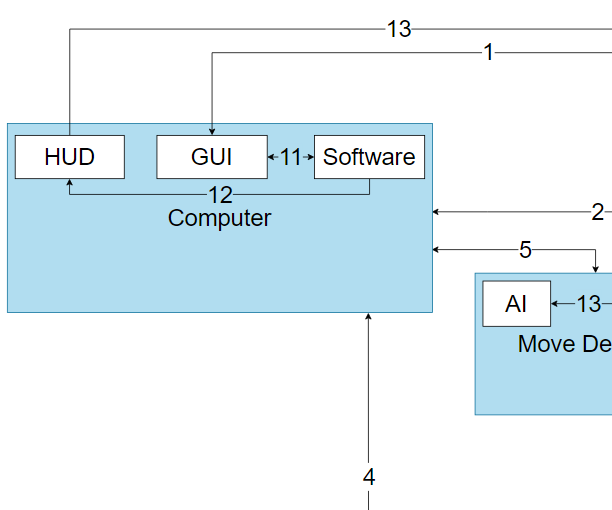
\includegraphics[width=0.80\textwidth]{images/computer_subsystems.png}
 \caption{Computer layer subsystems diagram}
\end{figure}

\subsubsection{Assumptions}
% Any assumptions made in the definition of the subsystem should be listed and described. Pay particular attention to assumptions concerning interfaces and interactions with other layers.

N/A
% The HUD information is able to be displayed on the computer screen to the user.

\subsubsection{Responsibilities}
% Each of the responsibilities/features/functions/services of the subsystem as identified in the architectural summary must be expanded to more detailed responsibilities. These responsibilities form the basis for the identification of the finer-grained responsibilities of the layer's internal subsystems. Clearly describe what each subsystem does.
The HUD subsystem displays to the user the status of the game and any information needed for the user. In this case the user is the Opponent layer. Information on the status of the game includes the current scores and a display of the game board on the computer monitor. This information is provided by the Software subsystem. When the physical game board changes, such as when a player moves a piece, this will also be reflected on the screen through the HUD.

\subsubsection{Subsystem Interfaces}
% Each of the inputs and outputs for the subsystem are defined here. Create a table with an entry for each labelled interface that connects to this subsystem. For each entry, describe any incoming and outgoing data elements will pass through this interface.

% \begin {table}[H]
% \caption {HUD Subsystem interfaces} 
% \begin{center}
%     \begin{tabular}{ | p{1cm} | p{6cm} | p{3cm} | p{3cm} |}
%     \hline
%     ID & Description & Inputs & Outputs \\ \hline
%     \#xx & Description of the interface/bus & \pbox{3cm}{input 1 \\ input 2} & \pbox{3cm}{output 1}  \\ \hline
%     \#xx & Description of the interface/bus & \pbox{3cm}{N/A} & \pbox{3cm}{output 1}  \\ \hline
%     \end{tabular}
% \end{center}
% \end{table}

Detailed in Table 2 are interfaces connected to the HUD subsystem. Incoming and outgoing data elements are detailed.

\begin {table}[H]
\caption {HUD Subsystem interfaces} 
\begin{center}
    \begin{tabular}{ | p{1cm} | p{6cm} | p{3cm} | p{3cm} |}
    \hline
    ID & Description & Inputs & Outputs \\ \hline
    \#12 & Information received from the Software subsystem to display & \pbox{3cm}{Game status and board} & \pbox{3cm}{N/A}  \\ \hline
    \#13 & Display game status through the Computer to the Opponent & \pbox{3cm}{N/A} & \pbox{3cm}{Game status and board}  \\ \hline
    \end{tabular}
\end{center}
\end{table}



\subsection{GUI Subsystem}
% Repeat for each subsystem
% This section should be a general description of a particular subsystem for the given layer. For most subsystems, an extract of the architectural block diagram with data flows is useful. This should consist of the subsystem being described and those subsystems with which it communicates.

The Graphical User Interface (GUI) subsystem is the main interactive component between the Computer and Opponent layers. It communicates with the Software subsystem within the Computer layer for its inputs and outputs.

\subsubsection{Assumptions}
% Any assumptions made in the definition of the subsystem should be listed and described. Pay particular attention to assumptions concerning interfaces and interactions with other layers.
The GUI only responds to keyboard inputs.

\subsubsection{Responsibilities}
% Each of the responsibilities/features/functions/services of the subsystem as identified in the architectural summary must be expanded to more detailed responsibilities. These responsibilities form the basis for the identification of the finer-grained responsibilities of the layer's internal subsystems. Clearly describe what each subsystem does.

The GUI is displayed on the monitor and can be interacted with by the use of keyboard keys by the player. These buttons will be able to change the state of the game for purposes such as new game, indicate their end of turn and quit game. Each time the opponent interacts with the GUI by sending a keyboard input for a specific function, this will interact with the computerized version of the game and update the game accordingly.

\subsubsection{Subsystem Interfaces}
% Each of the inputs and outputs for the subsystem are defined here. Create a table with an entry for each labelled interface that connects to this subsystem. For each entry, describe any incoming and outgoing data elements will pass through this interface.

Detailed in Table 3 are interfaces connected to the GUI subsystem. Incoming and outgoing data elements are detailed.

\begin {table}[H]
\caption {GUI Subsystem interfaces} 
\begin{center}
    \begin{tabular}{ | p{1cm} | p{6cm} | p{3cm} | p{3cm} |}
    \hline
    ID & Description & Inputs & Outputs \\ \hline
    \#1 & Opponent interacts with the GUI through keyboard inputs & \pbox{3cm}{Keyboard Input} & \pbox{3cm}{Game state change}  \\ \hline
    \#11 & Game state changes due to user interaction with the GUI & \pbox{3cm}{Keyboard Input} & \pbox{3cm}{Game state change}  \\ \hline
    \end{tabular}
\end{center}
\end{table}



\subsection{Software Subsystem}
% Repeat for each subsystem
% This section should be a general description of a particular subsystem for the given layer. For most subsystems, an extract of the architectural block diagram with data flows is useful. This should consist of the subsystem being described and those subsystems with which it communicates.

The Software subsystem is the main program behind the actions the UR5 Robot Arm will execute. This subsystem not only includes the source code itself, but also software packages needed for the program.

\subsubsection{Assumptions}
% Any assumptions made in the definition of the subsystem should be listed and described. Pay particular attention to assumptions concerning interfaces and interactions with other layers.
The subsystem is able to send instructions to the UR5 robot arm.

\subsubsection{Responsibilities}
% Each of the responsibilities/features/functions/services of the subsystem as identified in the architectural summary must be expanded to more detailed responsibilities. These responsibilities form the basis for the identification of the finer-grained responsibilities of the layer's internal subsystems. Clearly describe what each subsystem does.

The Software subsystem is responsible for handling events from the GUI. The subsystem also communicates with the UR5 robot arm through the Computer layer. The subsystem handles data on the status of the robot arm received from the robot arm itself. It also communicates to the robot arm what programmed actions it will need to perform. These actions will be determined by its interactions with the Move Decision layer which consists of the AI subsystem. The Software subsystem is also responsible for handling inputs from the Input Button/Device layer through the Computer layer.

\subsubsection{Software Subsystem Interfaces}
% Each of the inputs and outputs for the subsystem are defined here. Create a table with an entry for each labelled interface that connects to this subsystem. For each entry, describe any incoming and outgoing data elements will pass through this interface.

Detailed in Table 4 are related interfaces to the Software subsystem. Incoming and outgoing data elements are detailed.

\begin {table}[H]
\caption {Subsystem interfaces} 
\begin{center}
    \begin{tabular}{ | p{1cm} | p{6cm} | p{3cm} | p{3cm} |}
    \hline
    ID & Description & Inputs & Outputs \\ \hline
    \#2 & Signal that a turn has been completed by the Opponent & \pbox{3cm}{Keyboard Input pressed signal} & \pbox{3cm}{Signal to Move Decision layer}  \\ \hline
    \#4 & Communication between Move Execution and Computer layers & \pbox{3cm}{UR5 robot arm status} & \pbox{3cm}{Actions to be performed by the UR5 robot arm}  \\ \hline
    \#5 & Communication between Move Decision and Computer layers & \pbox{3cm}{Next move to make} & \pbox{3cm}{Game state change}  \\ \hline
    \#11 & Game state changes due to user interaction with the GUI & \pbox{3cm}{Keyboard Input signal} & \pbox{3cm}{Game state change}  \\ \hline
    \end{tabular}
\end{center}
\end{table}